\chapter{Le Magnétisme Moléculaire}

Pour mériter le nom d'aimant moléculaire, une molécule doit remplir plusieurs critères. Bien s\^ur, il faut qu'elle possède un moment magnétique non nul qui peut \^etre de spin et/ou orbital. Il faut de plus, que ce moment magnétique est une orientation préférentielle. Cela se traduit par l'existence d'un axe facile, c'est à dire deux orientations qui correspondent à un minimum d'énergie. En outre, l'anisotropie, c'est à dire la barrière d'énergie séparant les deux orientations, doit \^etre suffisamment grande pour que l'énergie thermique ne puisse pas retourner l'aimantation.

On souhaite aussi pouvoir mettre en évidence des phénomènes quantiques tel que le retournement de l'aimantation par effet tunnel~(ou Quantum Tunneling of the Magnetization - QTM~\cite{Thomas1996,Friedman1996}) ou bien encore la phase de Berry~\cite{Wernsdorfer1999}. Ceci n'est possible que s'il existe un couplage entre les différents états magnétiques. Celui-ci a généralement pour origine la présence d'un plan difficile qui va introduire des termes création/annihilation dans la description du système.

Le spin électronique n'est pas toujours l'unique acteur du magnétisme moléculaire. Il arrive que le spin nucléaire, au travers du couplage hyperfin, joue un r\^ole majeur dans les phénomènes quantiques et les propriétés magnétiques mesurées. C'est la cas notamment lorsque l'on s'intéresse au magnétisme des orbitales f où la géométrie de l'orbitale favorise l'interaction hyperfine.

Afin de comprendre la physique associée aux aimants moléculaires, on peut introduirons la notion d'axe facile et de plan difficile. Une description des interactions entre spin électronique et spin nucléaire est nécessaire pour décrire de la façon la plus complète certains aimants moléculaires, à base de lanthanide notamment.

\section{L'origine du moment magnétique}
Pour obtenir un aimant moléculaire, deux stratégies peuvent être adoptées. La première consiste à synthétiser une molécule composé de plusieurs atomes magnétique qui vont interagir entre eux, par l'intermédiaire des ligands, pour donner un moment magnétique résultant non nul. La deuxième ne nécessite qu'un atome métallique magnétique que l'on va venir insérer dans un ligand non magnétique.

\subsection{La solution à plusieurs centres}
Cette solution a été la première adoptée dans le domaine du magnétisme moléculaire. Elle a permis notamment de synthétiser la désormais célèbre molécule de Mn$_{12}$-ac~\cite{Lis1980}~(cf Fig.\ref{Mn12}). Cette dernière possède un coeur magnétique composé de douze atomes de Manganèse et d'autant d'atomes d'oxygène. Celui-ci est entouré par des ligands organiques. Les huit atomes de manganèse en périphérie, de part leur interaction, sont parallèles les uns au autres. Chacun d'eux possédant un spin $S=2$, le spin total résultant est $S=16$. Les trois atomes situés au centre du coeur magnétique sont également alignés entre eux pour un spin total de $S=6$~(pour chaque manganèse $S=3/2$). Ces deux groupes étant antiparallèles l'un par rapport à l'autre, on obtient un spin total de $S=10$. Dans cet exemple, les atomes d'oxygène jouent un r\^ole majeur au travers de l'interaction dite de "super échange" qui lie les différents atomes de Manganèse entre eux.
\begin{figure}
\centering 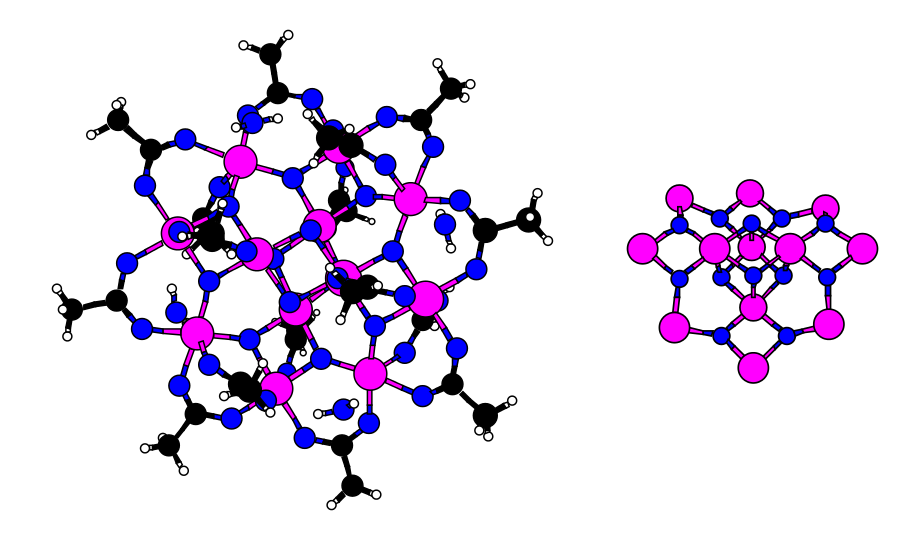
\includegraphics[scale=0.3]{Theorie/MagMol/figure1/Mn12.png} 
\caption{Sur la gauche, la molécule de Mn$_{12}$-ac. Sur la droite, le centre magnétique Mn$_{12}$O$_{12}$. Les quatre manganèses internes de spin $S=3/2$ sont antiparallèles aux huit maganèses de spin $S=2$ situés en périphérie. Le moment magnétique total résultant est $S=10$~(extrait de \cite{MagGoesNano}). Le couplage entre les différents spins est médié par les atomes d'oxygène en bleus sur la figure.}
\label{Mn12}
\end{figure}

\subsection{La solution de l'ion métallique unique}
Dans ce deuxième type d'aimants moléculaires, le moment magnétique total ne dépend que de celui de l'ion qui la compose. Ensuite, cet ion va \^etre inséré dans un ligand pour former un aimant moléculaire. Contrairement à ce qui a été présenté précédemment, le moment magnétique total ne dépend donc pas des interactions entre différents centres magnétiques. On peut d'ores et déjà y voir un signe de robustesse, ce type d'aimant moléculaire étant, par construction, moins sensible à une déformation de sa structure. Parmi les molécules les plus étudiées , on trouve le "double-decker"~(nommé en référence aux avions à deux ailes) où plusieurs ions peuvent \^etre choisis comme centre magnétique. Dans notre cas, nous utiliserons le TbPc$_2$~\cite{Ishikawa2005} ou terbium "double-decker".



\section{Hamiltonien d'un aimant moléculaire "standard"}
\subsection{L'axe facile}
Le champ de ligand a une influence majeure sur le magnétisme de la molécule. Celui-ci peut \^etre pris en compte par l'introduction des opérateurs de Stevens~\cite{Stevens1952}~(rappelé en annexe) qui tiennent compte des symétries du système. Pour notre introduction, nous allons nous concentrer sur un terme simple introduisant un axe facile à savoir:
 \begin{eqnarray}
E_{ani} = -DS_z^2 \nonumber
\end{eqnarray}
où $D$ est le paramètre d'anisotropie, $S_z$ la composante en $z$ du moment magnétique et $E_{ani}$ la modification de l'énergie du système d\^u à cette anisotropie. Si $D<0$, nous avons à faire à un axe difficile et le moment magnétique se trouvera de préférence dans le plan perpendiculaire à l'axe $z$. Si $D>0$, nous avons un axe facile et le moment magnétique sera aligné le long de l'axe z.

La Fig.\ref{Fe8Zeeman}.a présente la position en énergie des différents états $|m_z \rangle$ dans le cas $S=10$ et $D>0$. On remarque que les deux orientations préférentielles $m_z=10$~(up) et $m_z=-10$~(down) sont séparées par une barrière d'anisotropie de hauteur $|D|S^2$.

\begin{figure}
\centering 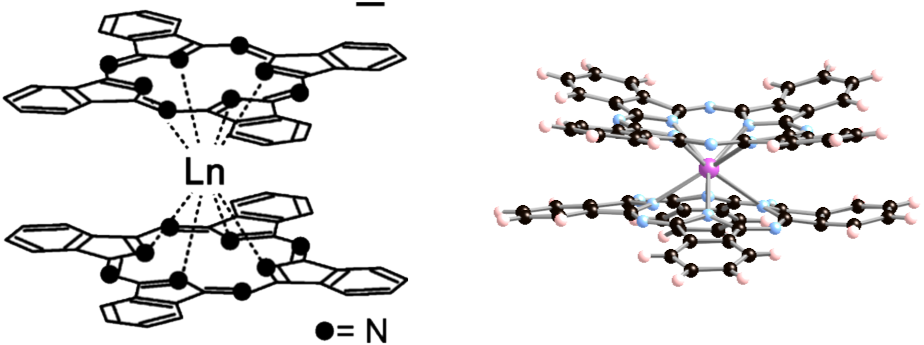
\includegraphics[scale=0.3]{Theorie/MagMol/figure2/figure2.png} 
\caption{A gauche, structure générale d'un "double decker" à base de Lanthanide~(noté Ln - tiré de Ishikawa, Single molecule magnet with single lanthanide ion). A droite, vu d'artiste de cette m\^eme molécule. Les atomes d'azote sont représentés en bleu, ceux de carbone en noir, ceux d'hydrogène en beige et l'atome lanthanide en mauve.}
\label{TbPc2}
\end{figure}

\subsection{Le plan difficile}
De m\^eme que nous pouvons avoir un axe facile~(ou difficile), on peut également rencontrer un plan difficile~(ou facile). Il peut \^etre exprimé de deux façons rigoureusement équivalentes :
\begin{eqnarray}
E_{\perp} = E ( S_x^2 -S_y^2)  = \frac{E}{2} ( S_+^2  + S_-^2) \nonumber 
\end{eqnarray}
où $S_x$ et $S_y$ sont les projections du moment magnétique dans le plan $(x,y)$, $S_+$ et $S_-$ les opérateurs création anhilation, $E$ est le paramètre d'anysotropie et $E_{\perp}$ l'énergie associée à la présence d'un plan difficile. La présence des termes création/anhilation n'est pas sans conséquence sur le système. En effet, ces termes vont venir coupler les différentes états $m_z$. Ceci conduit généralement à une physique plus riche et donc plus intéressante.

\subsection{L'effet Zeeman}
Comme tout système magnétique, un aimant moléculaire est sensible à l'effet Zeeman. Celui-ci va venir faire varier l'énergie du système de la valeur
\begin{eqnarray}
E_{z}= g\mu_b \mathbf{BS} \nonumber
\end{eqnarray}
ou $E_{z}$ est l'énergie associée à l'effet Zeeman, $g$ le facteur de Landé, $\mu_b$ le magnéton de Bohr, $B$ le champ magnétique appliqué et $S$ le moment magnétique du système. Si maintenant, ce champ magnétique est appliqué selon l'axe $z$ du système, cette expression devient :
\begin{eqnarray}
E_{z}= g\mu_b B S_z \nonumber
\end{eqnarray}

\subsection{La cas du Fe$_8$}
Si l'on synthétise ce qui vient d'\^etre présenté, un aimant moléculaire soumit à un champ magnétique $B$ appliqué suivant l'axe $z$ possède l'hamiltonien suivant:
\begin{eqnarray}
E =  -DS_z^2 + \frac{E}{2} ( S_+^2  + S_-^2) + g\mu_b B S_z 
\end{eqnarray}


On peut appliquer cet hamiltonien à l'étude d'un aimant moléculaire comme le Fe$_8$~\cite{Barra1996}, très utilisé dans les expériences de magnétisme moléculaire. Cet aimant possède un spin $S=10$ qui a pour origine l'interaction entre 8 atome de Fer. Les paramètres du champ de ligand sont fournis par \cite{Barra1996} et sont égaux à 46\,mK pour le plan difficile et 275\,mK pour l'axe facile. La Fig.\ref{Fe8Zeeman}.b présente son digramme Zeeman dans lequel les niveaux  de bas en haut vont de $m_z=\pm10$ à $m_z=0$. La zone grisée indique un croisement qui s'ouvre du fait de la présence d'un plan difficile. On désigne de telle zone par le terme d'anti-croisement~(cf Fig.\ref{Fe8Zeeman}). Nous allons maintenant détailler la physique de ces zones bien particulières.
\begin{figure}
\centering 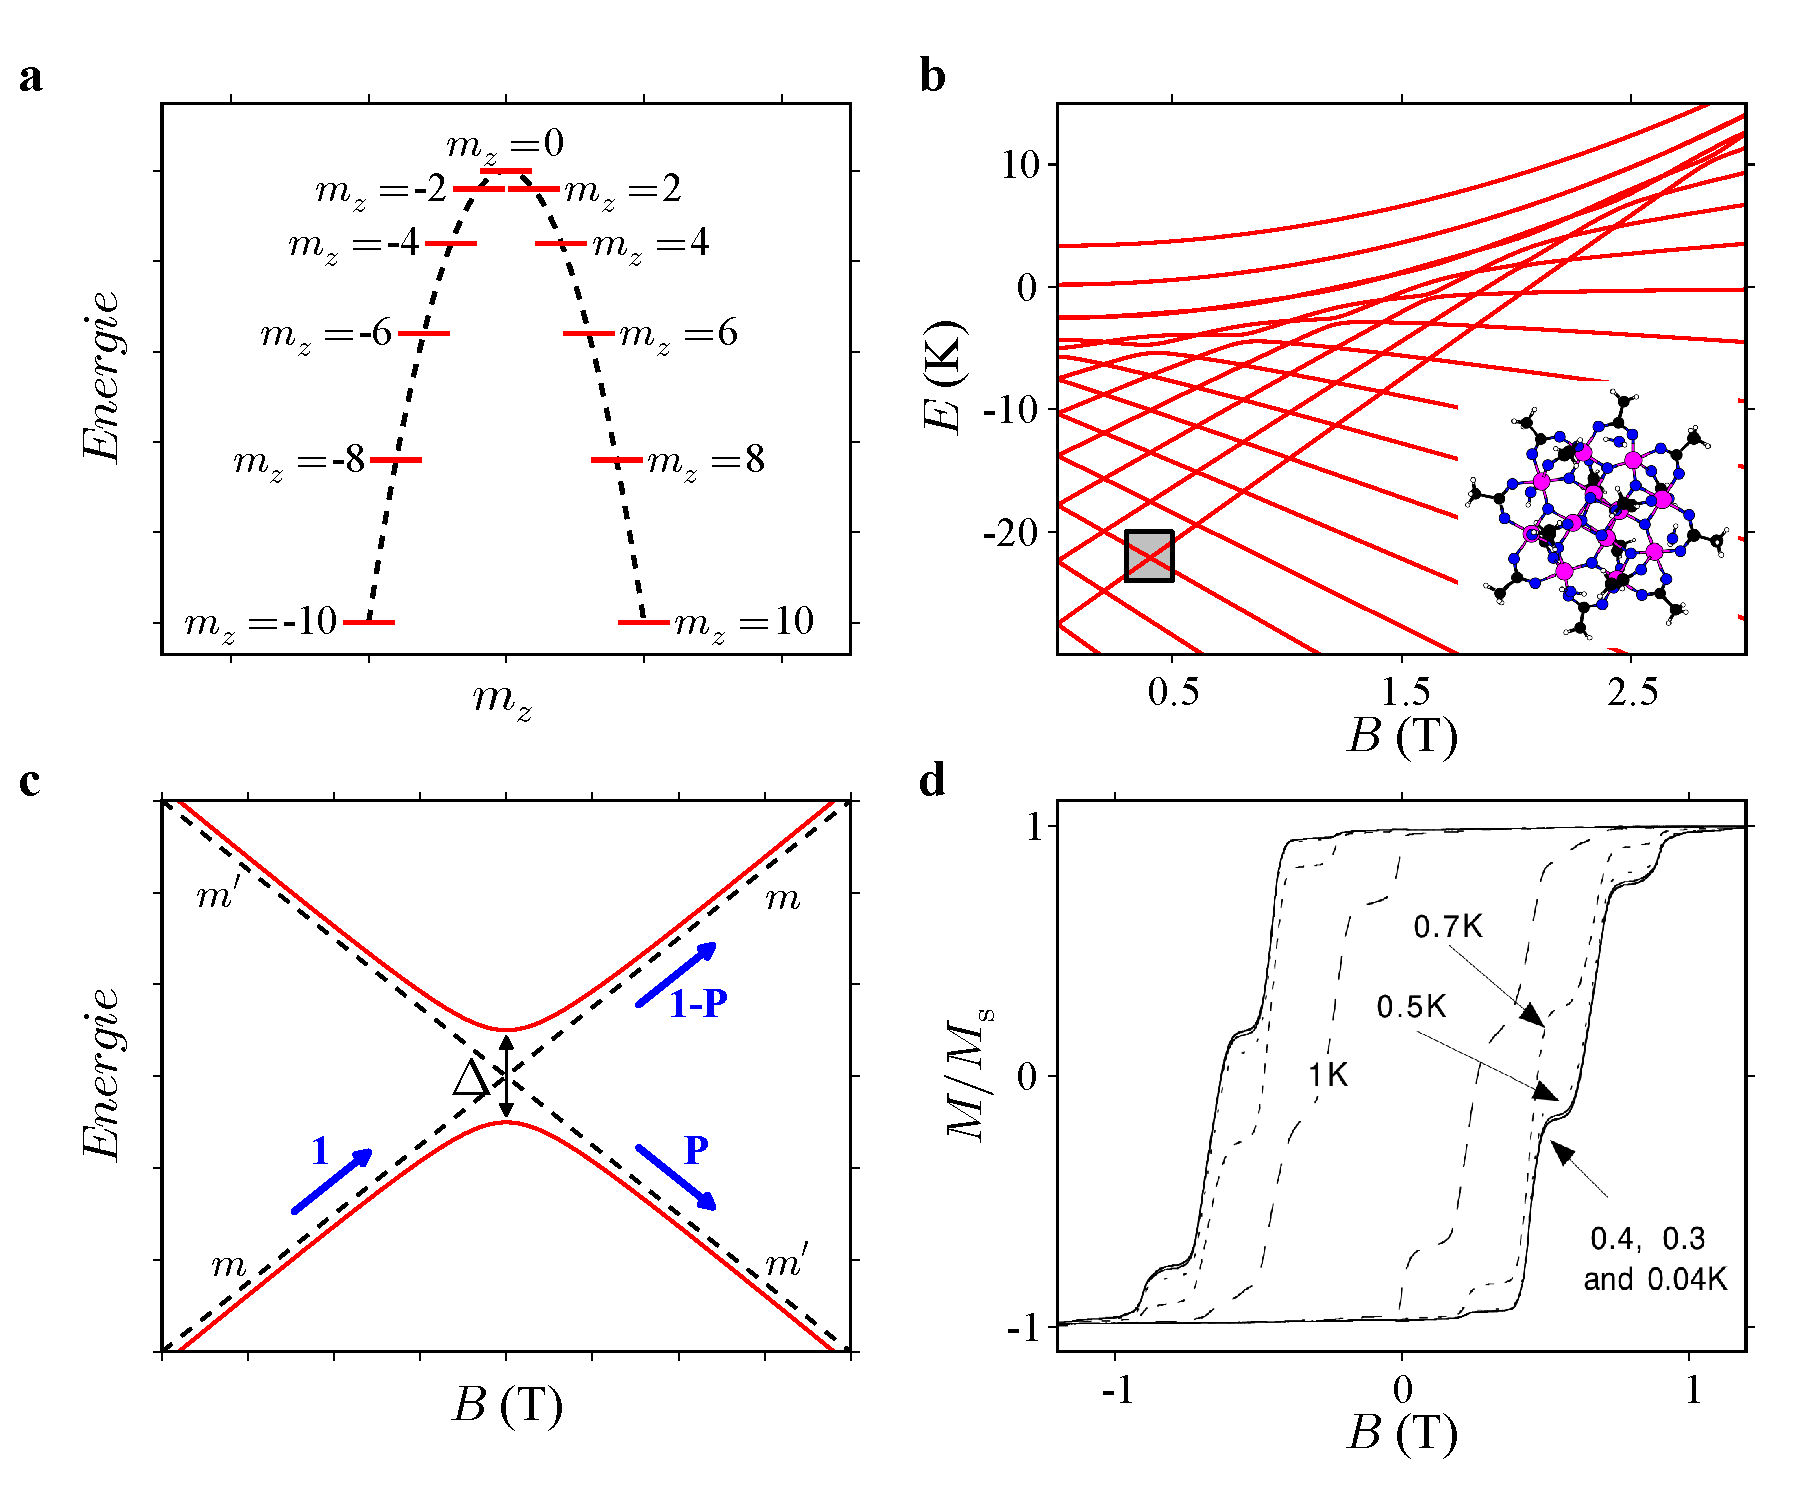
\includegraphics[scale=0.45]{Theorie/MagMol/figure3/figure3.pdf} 
\caption{\textbf{a} : énergie en fonction du nombre quantique $m_z$. Les deux orientations $m_z=\pm 10$ sont séparées par une barrière d'énergie de hauteur $|D|S^2$~\cite{Bogani2008}. \textbf{b} : diagramme Zeeman de la molécule Fe$_8$ représentant l'énergie des différents états du système en fonction du champ magnétique. Certains croisements, comme celui marqué d'un carré, sont en fait des anti-croisements traduisant un couplage entre les états. \textbf{c} : anti-croisement représentant un couplage entre les états $m$ et $m'$. \textbf{P} est la probabilité de transition entre les états $m$ et $m'$ lorsque l'on balaie l'anti-croisement en champ magnétique. \textbf{c} : mesure de l'aimantation d'un cristal de Fe$_8$ obtenue par technique micro-squid pour différentes températures. Les anti-croisements sont visibles à travers les marches qui traduisent un renversement de l'aimantation d'un grand nombre de molécules pour des valeurs particulières du champ magnétique~(extrait de \cite{MagGoesNano}).}
\label{Fe8Zeeman}
\end{figure}

\subsection{Les anti-croisements}
La géométrie d'un anti-croisement type est présenté dans la Fig.\ref{Fe8Zeeman}.c. La ligne en pointillé correspond au diagramme Zeeman en l'absence de plan difficile. Si l'on se place loin de l'anti-croisement, les états $m$ et $m'$ sont les états propre du système. Mais plus on se rapproche de l'anti-croisement plus les états se mélangent pour atteindre un maximum d'intrication quand la séparation en énergie entre les deux niveaux est minimale.

Lorsque l'on balaie le champ magnétique autour d'un tel anti-croisement, il y a une certaine probabilité de passer de l'état $m$ à l'état $m'$ et vice-versas. Cette probabilité est régie par la formule de Landau-Zener~\cite{Zener1932} qui dépend à la fois de la séparation minimale entre les deux niveaux~$\Delta_{mm'}$ ainsi que de la vitesse de balayage du champ magnétique~$\frac{dB_z}{dt}$. Cette probabilité peut s'exprimer de la façon suivante :
\begin{eqnarray}
P = 1 - \exp \left( -\frac{\pi \Delta^2_{mm'}}{2 \hbar g \mu_B |m-m'|\frac{dB_z}{dt}} \right)
\end{eqnarray}
ou P est la probabilité de passer de l'état $m$ à l'état $m'$. On constate tout d'abord que si la vitesse est très faible, la probabilité de passer d'un état à l'autre est de 1. On retrouve ici le théorème adiabatique. A l'autre bout de l'échelle, si je balaie très rapidement le champ magnétique cette probabilité devient nulle. Tout se passe comme si le système n'avait pas eu le temps de "sentir" l'anti-croisement.

\subsection{Mesure de l'aimantation}
Une manière de rendre compte des propriétés magnétiques des aimants moléculaires est de mesurer l'aimantation d'un cristal moléculaire en fonction du champ magnétique. Cette mesure est présentée dans le Fig.\ref{Fe8Zeeman}.d pour plusieurs températures et une vitesse de balayage de 14\,mT.s$^{-1}$. La courbe montre une série de marches qui sont d\^ues au retournement de l'aimantation par effet tunnel. Chacune d'elles correspond à un anti-croisement sur lequel l'aimantation à une probabilité élevée de transiter. Lorsque l'on diminue la température, le taux de retournement diminue car les transitions assistées thermiquement diminuent. Cette courbe devient indépendante de la température au dessous de 400\,mK et on observe les transitions correspondantes aux niveaux de plus basse énergie. 


\section{Le Terbium double-decker ou TbPc$_2$}

\subsection{Origine du moment magnétique}
Le terbium double-decker est un aimant moléculaire dont le moment magnétique est d\^u à un centre magnétique unique : l'ion Tb$^{3+}$. L'atome de Terbium possède un noyau relativement lourd et le couplage spin orbite joue un r\^ole prépondérant dans les propriétés magnétiques de ce dernier. Le moment magnétique fondamental total de cet ion peut \^etre déterminé par un calcul relativement complexe. La théorie donne un moment total $J=6$ pour l'état fondamental ainsi qu'une séparation en énergie de plusieurs milliers de Kelvin entre celui-ci et le premier état excité $J=5$. On peut, sans trop de risque, négliger les états excités et considérer uniquement la configuration $J=6$. Ce moment provient du moment angulaire électronique~($L=3$) ainsi que des six spins électroniques non appariés. 

\begin{figure}
\centering 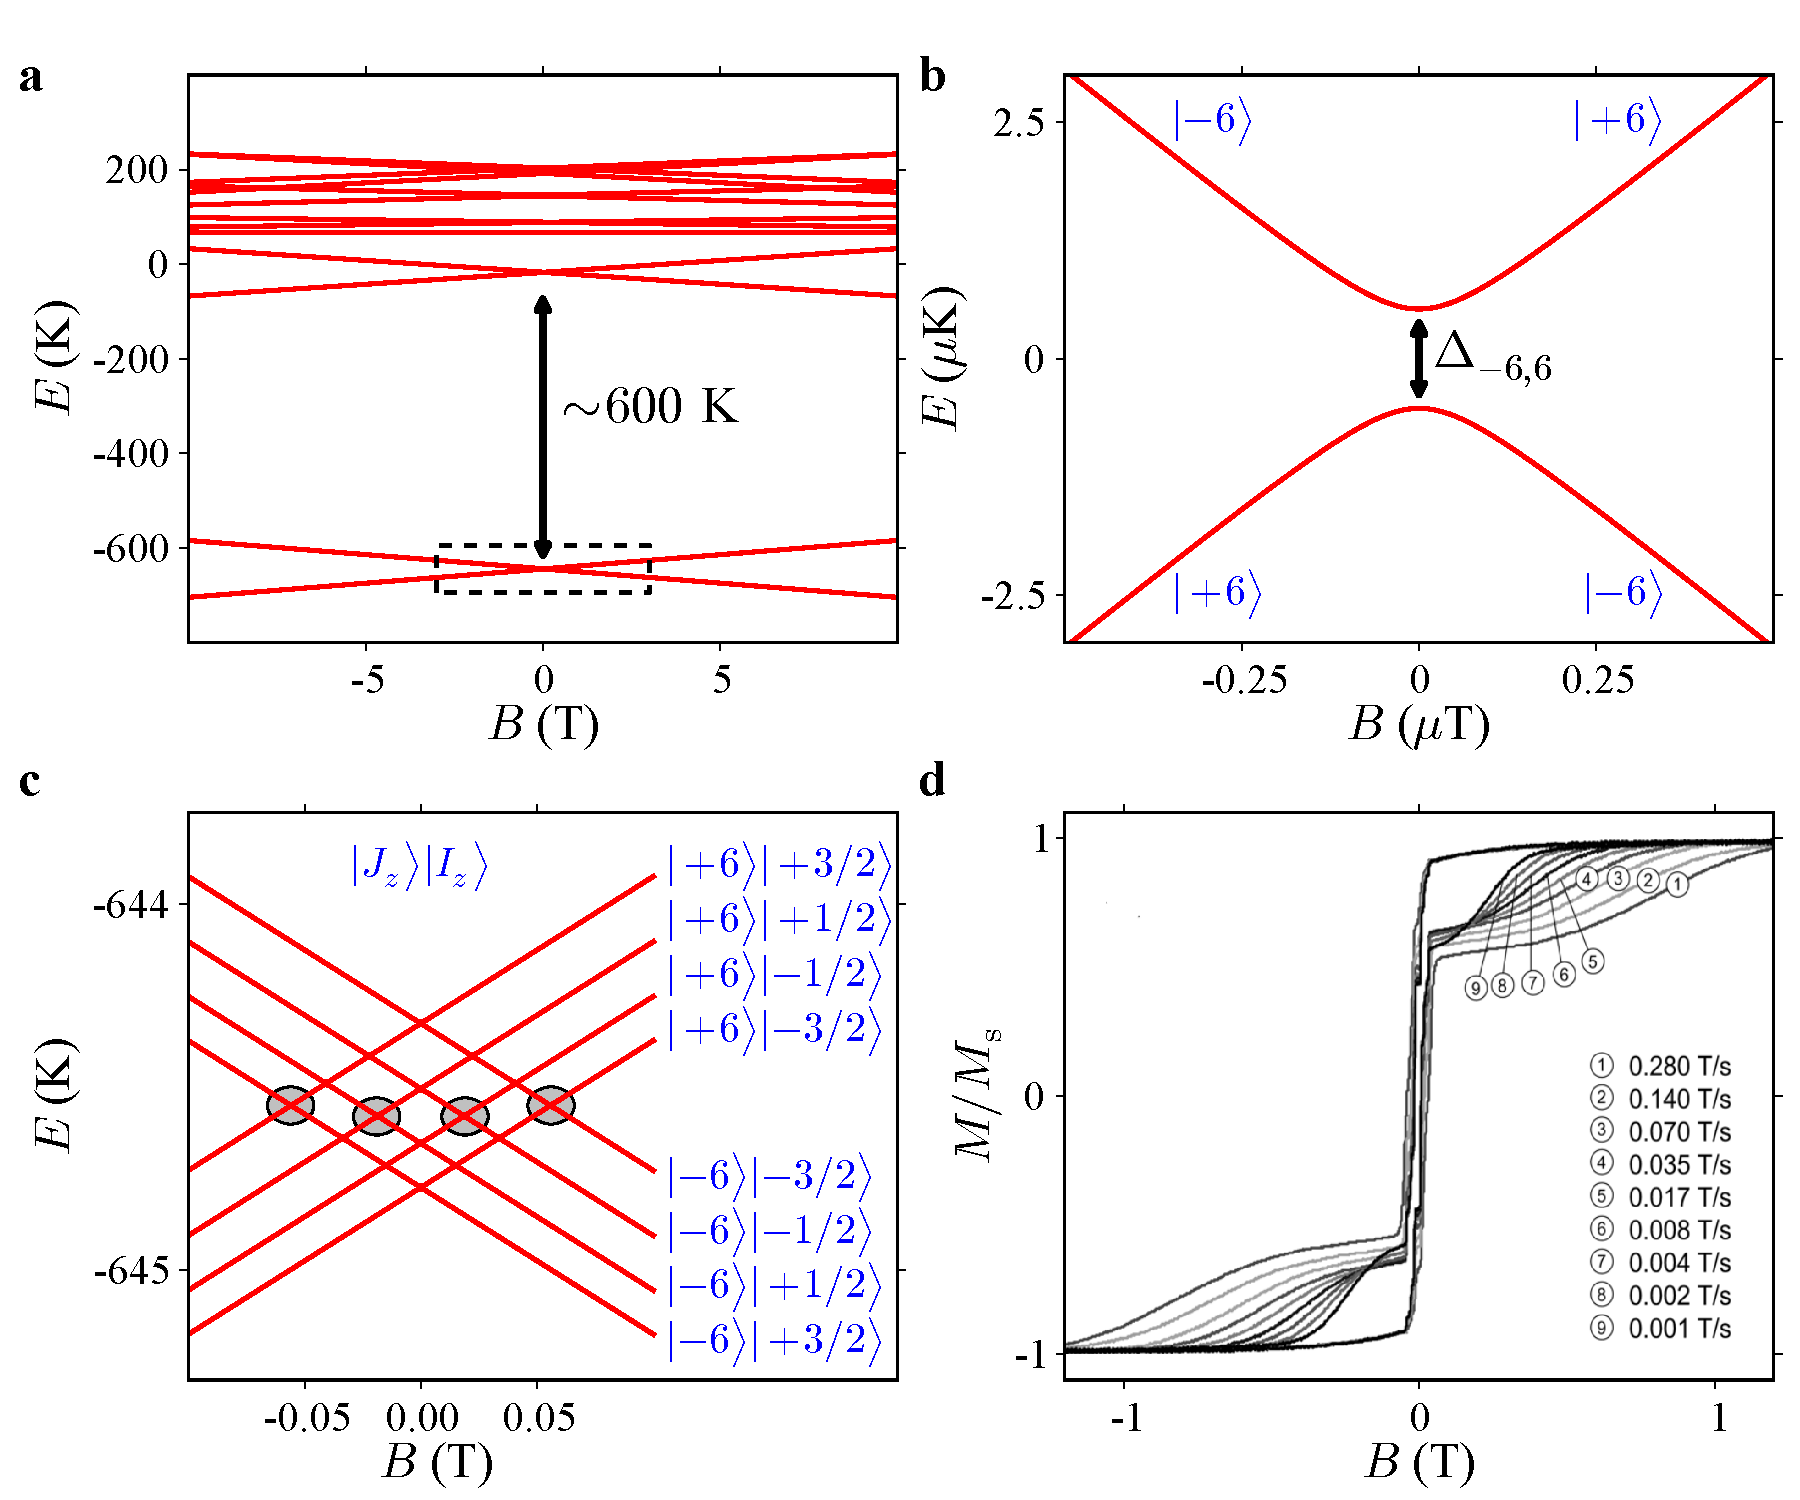
\includegraphics[scale=0.45]{Theorie/MagMol/figure4/figure4.pdf} 
\caption{\textbf{a} : diagramme Zeeman de la molécule TbPc$_2$ représentant l'énergie des différents états du système en fonction du champ magnétique. Les états fondamentaux $J_z \pm 6$ sont séparés des premiers états excités par une énergie de $600$\,K. A basse température, on peut se concentrer sur les états fondamentaux. \textbf{b} : Agrandissement du diagramme Zeeman des deux états fondamentaux à faible champ magnétique. Il met en évidence un anti-croisement de valeur minimale $\Delta_{-6,6}$ de l'ordre du $\mu$K qui traduit une intrication entre les deux états.\textbf{c} : Diagramme Zeeman lorsque l'on tient compte du couplage hyperfin avec le spin $I=3/2$ du noyau. On ne relève que quatre anti-croisements marqués d'un cercle qui sont autant de zone ou les états $J_z =\pm6$ sont intriqués. \textbf{d} : Mesure de l'aimantation d'un cristal de TbPc$_2$ obtenu par technique micro-squid. Les molécules se retournent majoritairement à faible champ, ce qui correspond à quatre anti-croisements présentés dans \textbf{c}~(inspiré de \cite{Ishikawa2005}).}
\label{TbPc2Zeeman}
\end{figure}

\subsection{Hamiltonien}

\subsubsection{Le moment magnétique électronique}
L'Hamiltonien relatif au TbPc$_2$ est plus complexe que ce qui a été présenté précédemment. Il est pour cela plus pratique de faire appel aux opérateurs de Stevens afin d'obtenir une écriture plus concise.

L'Hamiltonien relatif à la présence d'un axe facile s'exprime comme suit :
\begin{eqnarray}
H_{//} = \alpha A_2^0 \langle r^2 \rangle O_2^0 + \beta A_4^0 \langle r^2 \rangle O_4^0 + \gamma A_6^0 \langle r^2 \rangle O_6^0
\end{eqnarray}
ou les différents $O_i^0$ sont les opérateurs de Stevens, $A_i^0$ les coéfficients relatifs à la molécule de TbPc$_2$~\cite{Ishikawa2005} et $\alpha$, $\beta$ et $\gamma$ les coéfficients introduits par Stevens. Les opérateurs $O^0_i$ sont basés sur des sommes d'opérateurs $S_z^{2n}$. Il s'agit donc d'un opérateur diagonal qui ne vient pas coupler les différents états de la base ($J$,$J_z$) entre eux. Le diagramme Zeeman correspondant est donné dans la Fig.\ref{TbPc2Zeeman}.a.

Les états fondamentaux $J_z = \pm 6$ sont isolés des états excités par une énergie de plus de $600$\,K. Puisque nos expériences se font dans le domaine du sub-Kelvin, on peut négliger les états excités et nous concentrer sur les deux états fondamentaux  $J_z = \pm 6$.

La présence d'un plan difficile, nécessite l'introduction d'un terme suplémentaire :
\begin{eqnarray}
H_{\perp} = \beta A_4^4 \langle r^2 \rangle O_4^4
\end{eqnarray}
où la m\^eme notation a été utilisée. Ce dernier terme ne modifie pas l'allure générale du diagramme Zeeman. En revanche, il introduit un couplage entre les états  $J_z = \pm 6$ qui se traduit par la présence d'anti-croisement comme le montre la figure\ref{TbPc2Zeeman}.b.

\subsubsection{Le spin nucléaire}
Dans le cas du terbium, le spin nucléaire est de $I = 3/2$. Du fait de sa forme allongée, il possède également un moment quadripolaire de sorte que l'hamiltonien relatif au spin nucléaire est donné par~\cite{Bleaney1961} :
\begin{eqnarray}
H_I = P\left(I_z^2 - \frac{1}{3}I(I+1)\right)
\end{eqnarray}
où $P$ est le moment quadripolaire du spin nucléaire.

Les orbitale électronique étant de type 4f, le couplage hypefin doit \^etre pris en compte. Un terme rendant compte de cette interaction doit donc \^etre introduit. Son expression est simple et ne met en jeu que le produit scalaire des deux spins :
\begin{eqnarray}
H_{hf} = A_{hf}\mathbf{J}\mathbf{I}
\end{eqnarray}
où $\mathbf{J}$ et $\mathbf{I}$ sont respectivement le moment magnétique électronique et le spin nucléaire, $A_{hf}$ étant la constante d'interaction hyperfine.

\subsubsection{L'Hamiltonien de l'aimant moléculaire}

Ces différents terme doivent bien s\^ur \^etre inclus dans l'Hamiltonien total de l'aimant moléculaire. Cela donne, en reprenant la notion précédente :
\begin{eqnarray}
H = H_z + H_{//} + H_{\perp} + H_{hf} + H_I
\end{eqnarray}
Les trois derniers opérateurs agissent comme une perturbation et l'allure générale présenté dans la Fig.\ref{TbPc2Zeeman}.a n'est pas altéré. On peut donc continuer à ce concentrer sur les seuls états $J_z = \pm 6$. A cette échelle en revanche, les effets ne sont plus négligeables. En plus de l'anti-croisement introduit par la présence du plan difficile, le couplage hyperfin vient diviser les états fondamentaux  $J_z = \pm 6$ en deux jeux de quatre états, chacun de ces quatre états étant relatif à un état de spin nucléaire. De plus, pour un m\^eme état de spin nucléaire, l'anti-croisement entre les états de  $J_z = \pm 6$ est conservé. En revanche, seul des croisements sont observés pour les croisements entre les état de spins nucléaires différents~(cd Fig. \ref{TbPc2Zeeman}.c).

\subsection{Mesure de l'aimantation}
Une mesure de l'aimantation d'un cristal de TbPc$_2$ pour différentes vittessses de balayage est présentée dans la Fig.\ref{TbPc2Zeeman}.d. Une analyse détaillée peut \^etre trouvé dans \cite{Ishikawa2005}. On peut diviser la courbe en deux zones. A faible champ, les molécules constituant le cristal se retournent par QTM. Les marches que l'on devine correspondent à la zone du diagramme Zeeman présentée dans la Fig.\ref{TbPc2Zeeman}.c et le retournement est gouverné par la formule de Landau-Zener. Il dépend donc de la vitesse ce qui conduit à une variation de la hauteur des marches en fonction de la vitesse de balayage. A plus fort champ, l'aimantation ne peut se retourner qu'en émettant un phonon d'où la zone de transition continue. L'influence de la vitesse de balayage n'est dans ce cas pas d\^u à un effet Landau-Zener mais à un effet que l'on nomme Phonon-Bottleneck. Il rend compte du fait qu'un trop grand nombre de molécules "souhaitent" se retourner pour que toutes puissent émettre un phonon.